\chapter{Near the Horizon}

These notes follow Leonard Susskind's seventh lecture on general relativity in the order in which the blackboard argument unfolds. We begin by stripping the Schwarzschild metric down to a dimensionless form, then use that simplification to estimate curvature, introduce proper distance from the horizon, and finally turn the geometry into causal questions about what Alice, Bob, and Charlie actually see. The present companion-note draft credits Leonard Susskind, LazyingArt LLC, and Video2Book for the lecture and its curation.

\section{Rescaled Schwarzschild Geometry}

We begin exactly where the lecture begins: with the Schwarzschild metric itself. Susskind first writes it with primed variables, only so that he can rescale them and then drop the primes. With \(r_{\mathrm S}=2MG\), the standard form is
\begin{equation}
d\tau^2
=
\left(1-\frac{2MG}{r'}\right)dt'^2
-
\frac{dr'^2}{1-\frac{2MG}{r'}}
-
r'^2\,d\Omega_2^2.
\end{equation}
He then defines
\begin{equation}
r=\frac{r'}{r_{\mathrm S}},
\qquad
t=\frac{t'}{r_{\mathrm S}},
\qquad
r_{\mathrm S}=2MG.
\end{equation}
Because we are using units with \(c=1\), time and length carry the same dimensions, so both rescalings are natural. Substituting \(r'=r_{\mathrm S}r\) and \(t'=r_{\mathrm S}t\), we find
\begin{equation}
d\tau^2
=
r_{\mathrm S}^2
\left[
\left(1-\frac{1}{r}\right)dt^2
-
\frac{dr^2}{1-\frac{1}{r}}
-
r^2\,d\Omega_2^2
\right].
\end{equation}

\begin{remark}
A sign issue was caught from the room while the metric was being written on the board. We record only the corrected form above. The lecture also writes the angular line element in a convention-dependent way, but the discussion here never depends on that detail, so \(d\Omega_2^2\) is the safest notation.
\end{remark}

This is the first real payoff of the lecture. All Schwarzschild black holes have the same dimensionless metric. The only trace of their actual size is the overall factor \(r_{\mathrm S}^2\). That is why Susskind immediately says that, for purposes of geometry, we can study the unit black hole with \(r_{\mathrm S}=1\). It is the same move one makes with spheres: all spheres have the same metric up to an overall scale.

\section{Curvature Scale at the Horizon}

With the metric normalized, Susskind turns at once to physics. He does not compute the full curvature tensor. Instead he asks a sharper question: what can its size possibly be near the horizon?

The dimensional argument is short and decisive:
\begin{align}
[g_{\mu\nu}] &= 1,\\
[\Gamma] &\sim L^{-1},\\
[\mathcal R] &\sim L^{-2}.
\end{align}
The metric is dimensionless because it multiplies \(dx^\mu dx^\nu\), which already carries the dimensions of length squared. A Christoffel symbol contains one derivative with respect to position, so it scales like inverse length. The curvature tensor contains either a derivative of \(\Gamma\) or a product \(\Gamma^2\), and therefore has units of inverse length squared.

Now ask the question at the horizon, where \(r=1\). In the rescaled metric the only remaining quantity with dimensions is \(r_{\mathrm S}\). Therefore the curvature at the horizon must be of order
\begin{equation}
\mathcal R_{\text{horizon}} \sim \frac{1}{r_{\mathrm S}^2}.
\end{equation}
More generally, at any fixed dimensionless \(r\), curvature must have the form
\begin{equation}
\mathcal R(r)\sim \frac{1}{r_{\mathrm S}^2}\,f_{\mathcal R}(r),
\end{equation}
for some dimensionless function \(f_{\mathcal R}(r)\).

This is where the lecture immediately cashes the calculation out into physics. A larger black hole has a larger Schwarzschild radius, hence a smaller curvature at its horizon. Therefore the tidal forces at the horizon of a very large black hole are milder than those at the horizon of a small black hole. The horizon is a point of no return, but it need not be a locally violent place.

For orientation, Susskind later gives the physical scale: a solar-mass black hole, with Schwarzschild radius of order a kilometer, has fierce tidal forces near the horizon; a supermassive black hole can have horizon tidal forces small enough that an ordinary person would notice nothing dramatic at crossing.

\section{Proper Distance From The Horizon}

Having made that point, the lecture deliberately narrows focus. We now ignore the angular factor for a while and study the radial-time geometry of the unit black hole. The next move is to replace the coordinate \(r\) by something with a more immediate geometric meaning: proper distance from the horizon.

\begin{figure}[htbp]
\centering

\includegraphics[width=0.76\textwidth]{lecture_07_figure_02.png}
\caption{Blackboard sketch of the rescaled radial coordinate, with the horizon marked at \(r=1\).}
\end{figure}

\begin{figure}[htbp]
\centering
\begin{tikzpicture}[scale=1.1]
\draw[->] (0,0) -- (8,0) node[below] {$r$};
\fill (0,0) circle (1.2pt) node[below] {$0$};
\draw (2.4,0.14) -- (2.4,-0.14);
\draw (2.4,0.38) node[above] {horizon};
\draw (2.4,-0.34) node[below] {$1$};
\end{tikzpicture}
\caption{Clean redraw of the radial line used to define proper distance from the horizon.}
\end{figure}

The point is that \(r-1\) is not the proper distance from the horizon. It is only a coordinate difference. To obtain actual distance, we freeze time and angles and move radially. On such a slice,
\begin{equation}
dt=0,
\qquad
d\Omega_2^2=0,
\end{equation}
and the metric gives
\begin{equation}
ds^2=\frac{dr^2}{1-\frac{1}{r}}.
\end{equation}
Taking the square root,
\begin{equation}
ds=\frac{dr}{\sqrt{1-\frac{1}{r}}}.
\end{equation}
Now use
\begin{equation}
1-\frac{1}{r}=\frac{r-1}{r},
\end{equation}
so that
\begin{equation}
ds=\sqrt{\frac{r}{r-1}}\,dr.
\end{equation}
This is the differential proper distance associated with a radial displacement \(dr\). Therefore the proper distance from the horizon to the point \(r\) is
\begin{equation}
\rho(r)=\int_1^r \sqrt{\frac{r'}{r'-1}}\,dr'.
\end{equation}

This is the central mathematical construction of the lecture. The lower limit is \(1\) because \(r=1\) is the horizon in the rescaled coordinates. The upper limit is the point whose distance from the horizon we want. Susskind remarks that the integral can be done, but he does not need its closed form. What matters is the geometric meaning of \(\rho\): it is the actual radial proper distance from the horizon.

We can also differentiate the definition immediately:
\begin{equation}
\frac{d\rho}{dr}=\sqrt{\frac{r}{r-1}},
\qquad\text{hence}\qquad
d\rho^2=\frac{dr^2}{1-\frac{1}{r}}.
\end{equation}
That identity is the reason for the entire change of variables.

\section{The Metric In \(\rho\) And \(\omega\)}

Once \(\rho\) has been introduced, the radial term collapses to the simplest possible form. Susskind then makes one more mild definition,
\begin{equation}
\omega=\frac{t}{2}.
\end{equation}
He is quite explicit that this is only a convenience. The factor of \(2\) is not deep physics; it is a normalization that makes the later formulas cleaner.

The blackboard form of the metric, supported directly by the lecture frame, is

\begin{figure}[htbp]
\centering

\includegraphics[width=0.82\textwidth]{lecture_07_figure_03.png}
\caption{Blackboard form of the metric in \((\rho,\omega)\) variables, together with the far-field limit.}
\end{figure}

\begin{equation}
d\tau^2
=
F(\rho)\rho^2\,d\omega^2
-
d\rho^2
-
r(\rho)^2\,d\Omega_2^2.
\end{equation}
Here \(F(\rho)\) is defined implicitly by rewriting the original coefficient of \(dt^2\) as a function of \(\rho\), and by splitting off a factor of \(\rho^2\). Susskind emphasizes that the split into \(F(\rho)\rho^2\) is initially arbitrary; the reason for it will become clear in the near-horizon limit.

The radial piece is now transparent. Since \(\rho\) was defined as proper distance, the second term is simply \(-d\rho^2\). The first term carries the nontrivial time dependence, but only through the coefficient \(F(\rho)\rho^2\).

Two limits matter:
\begin{equation}
\lim_{\rho\to\infty}F(\rho)\rho^2=4,
\qquad
\lim_{\rho\to 0}F(\rho)=1.
\end{equation}
The first expresses the fact that far from the black hole the geometry approaches the expected asymptotic form, with the factor of \(4\) coming from the choice \(\omega=t/2\). The second is the crucial one: close to the horizon, \(F(\rho)\) approaches \(1\).

There is also a near-horizon expansion for the inverse function \(r(\rho)\):
\begin{equation}
r(\rho)=1+\frac{\rho^2}{4}+\cdots.
\end{equation}
This is only a local expansion near \(\rho=0\), not an exact identity.

Therefore, near the horizon, the metric becomes
\begin{equation}
d\tau^2
\approx
\rho^2\,d\omega^2
-
d\rho^2
-
d\Omega_2^2.
\end{equation}
If we ignore the angular sphere for the moment, the radial-time part is
\begin{equation}
d\tau^2_{\text{radial-time}}
\approx
\rho^2\,d\omega^2-d\rho^2.
\end{equation}
This is exactly the flat Minkowski metric written in hyperbolic polar coordinates. The lecture does not insist on the full textbook transformation, but it is useful to recall the familiar flat-space relations
\begin{equation}
X=\rho\cosh\omega,
\qquad
T=\rho\sinh\omega,
\end{equation}
for which
\begin{equation}
dT^2-dX^2=\rho^2\,d\omega^2-d\rho^2.
\end{equation}
So the near-horizon region is locally flat spacetime in a coordinate system adapted to accelerated observers.

\section{Horizon, Interior, And Singularity}

Now the lecture turns from algebra to geometry. In the hyperbolic picture, lines of constant \(\rho\) are hyperbolae, and lines of constant \(\omega\) are rays. The horizon is \(\rho=0\), but in this geometry \(\rho=0\) is not a single point. It is the whole null line. Equivalently, \(\omega=\infty\) lies along the horizon.

\begin{figure}[htbp]
\centering
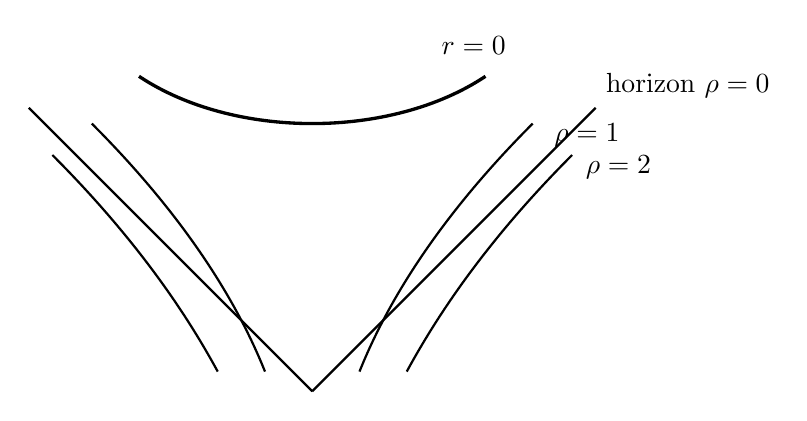
\begin{tikzpicture}[scale=1.0]
\draw[thick] (0,0) -- (3.6,3.6) node[above right] {horizon \(\rho=0\)};
\draw[thick] (0,0) -- (-3.6,3.6);
\draw[thick] (0.6,0.25) .. controls (0.9,1.0) and (1.5,2.1) .. (2.8,3.4);
\draw[thick] (1.2,0.25) .. controls (1.5,0.8) and (2.1,1.8) .. (3.3,3.0);
\draw[thick] (-0.6,0.25) .. controls (-0.9,1.0) and (-1.5,2.1) .. (-2.8,3.4);
\draw[thick] (-1.2,0.25) .. controls (-1.5,0.8) and (-2.1,1.8) .. (-3.3,3.0);
\draw[very thick] (-2.2,4.0) .. controls (-1.0,3.2) and (1.0,3.2) .. (2.2,4.0);
\draw (2.95,3.25) node[right] {\(\rho=1\)};
\draw (3.35,2.85) node[right] {\(\rho=2\)};
\draw (2.05,4.15) node[above] {\(r=0\)};
\end{tikzpicture}
\caption{Cautious reconstruction of the near-horizon causal picture. The horizon is the null line \(\rho=0\), and the singularity appears as the curve \(r=0\).}
\end{figure}

This is one of the conceptual turning points of the lecture. In ordinary Euclidean intuition, a small radius means a small circle shrinking toward a point. Here, by contrast, a tiny positive \(\rho\) corresponds to a hyperbola very close to a null line. As \(\rho\to 0\), the constant-\(\rho\) hyperbolae approach the entire lightlike horizon.

Inside the horizon, \(r<1\). In Susskind's discussion this corresponds to
\begin{equation}
r>1 \Longleftrightarrow \rho^2>0,
\qquad
r<1 \Longleftrightarrow \rho^2<0.
\end{equation}
He is careful about the interpretation: this sign flip is a coordinate artifact. It is not an invariant statement that space has literally turned into time or time into space. It means only that the coordinates are behaving differently across the horizon.

What is invariant is the causal structure. Once a timelike or null worldline crosses the horizon, the best it can do is still stay inside the future light cone. But inside the horizon all future-directed motion leads toward smaller \(r\), and eventually toward
\begin{equation}
r=0.
\end{equation}
That is not a coordinate singularity. It is a genuine curvature singularity. Tidal forces diverge there. No timelike or null worldline inside the horizon can avoid it, and it is reached in a finite amount of proper time.

At this point Susskind uses the name ``Kruskal coordinates.'' In the present lecture the important thing is not a full textbook derivation of the Kruskal map, but the smooth causal picture that the new coordinates reveal: \(r=1\) is not itself a dangerous place, while \(r=0\) is.

\section{Alice, Bob, Charlie, And The Rule: Draw The Diagram}

Only after the geometry is in place does the lecture introduce the observer stories. This is essential to the rhythm. Alice, Bob, and Charlie are not ornaments; they are tests of the causal diagram.

\begin{figure}[htbp]
\centering

\includegraphics[width=0.82\textwidth]{lecture_07_figure_04.png}
\caption{Blackboard sketch of Alice's infall, with the constant-time lines crowding against the limiting line \(t=\infty\).}
\end{figure}

\begin{figure}[htbp]
\centering
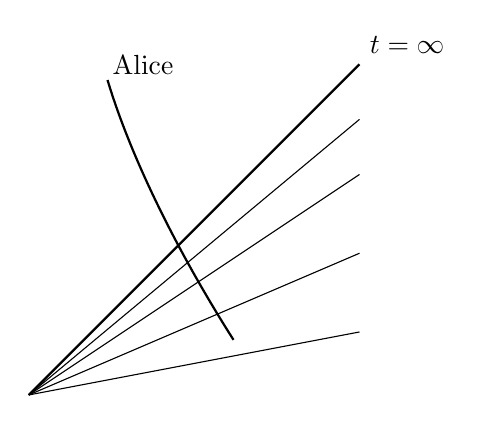
\begin{tikzpicture}[scale=1.0]
\draw[thick] (0,0) -- (4.2,4.2) node[above right] {\(t=\infty\)};
\draw[thin] (0,0) -- (4.2,0.8);
\draw[thin] (0,0) -- (4.2,1.8);
\draw[thin] (0,0) -- (4.2,2.8);
\draw[thin] (0,0) -- (4.2,3.5);
\draw[thick] (1.0,4.0) .. controls (1.3,3.0) and (1.9,1.8) .. (2.6,0.7);
\draw (1.45,3.95) node[above] {Alice};
\end{tikzpicture}
\caption{Simplified redraw of the causal sketch: constant Schwarzschild-time lines pile up against the horizon, while Alice's free-fall worldline passes through.}
\end{figure}

\subsection{Question \& Answer}

\paragraph{Question.} Why does Alice cross the horizon in finite proper time if the horizon sits at \(t=\infty\)?

\paragraph{Answer.} Because \(t\) is not Alice's clock. In the coordinate system tied to the exterior Schwarzschild description, the horizon is the limiting surface \(t=\infty\), or more precisely \(\omega=\infty\). But Alice's own proper time is measured along her worldline, and in that time nothing singular happens at the crossing. The diagram makes the distinction visible: the constant-time lines bunch up against the horizon, but Alice's worldline goes straight through.

This is not merely an abstract coordinate statement. Bob, who remains outside at fixed distance from the black hole, actually sees the same effect. He receives light from Alice along null rays, and every later ray he receives comes from a point on Alice's worldline closer to the horizon. If Bob stays outside forever, he sees Alice approach the horizon asymptotically and never sees her cross it. So ``the horizon is at \(t=\infty\)'' is exactly the statement about what the outside observer sees.

But that does not mean Alice fails to cross. It means only that once she has crossed she can no longer send a signal back out telling Bob that she has done so.

\subsection{Question \& Answer}

\paragraph{Question.} If Bob sees Alice slow down, does Alice see Bob speed up?

\paragraph{Answer.} No. This is one of the main traps the lecture wants us to avoid. Bob sees Alice slow down because he remains outside the horizon and receives light from Alice later and later, with her clocks appearing to run more and more slowly. But Alice, looking back at Bob, does not see some reciprocal runaway of Bob's clock.

What she sees is much more ordinary. She sees Bob in her past, just as everyone sees everyone else in the past because all sight is along light cones. She continues to see Bob without anything especially dramatic happening to him. What ends the story is not a catastrophe on Bob's worldline. What ends it is that Alice's worldline itself terminates at the singularity.

This is the lecture's geometric asymmetry. Bob can continue to receive signals from Alice only until she reaches the horizon; after that there are no outgoing signals from her to him. Alice, by contrast, can continue to see Bob for a while after she crosses the horizon, until she herself is destroyed.

The lecture sharpens this point with a vivid statement. If Bob stays outside forever, he sees Alice for an infinite amount of his time, but he sees only a finite number of heartbeats. In that limited sense he may say that Alice ``dies at the horizon,'' but only as an observational description tied to his accelerated frame. In her own proper time she is perfectly ordinary at the horizon and only runs into trouble near the singularity.

\subsection{Question \& Answer}

\paragraph{Question.} What does Charlie see if he follows Alice in free fall?

\paragraph{Answer.} Charlie sees nothing special at the horizon. This is the cleanest operational test of the claim that the horizon is locally mild for a large black hole. If Charlie falls just behind Alice, both of them are in free fall. They can exchange light signals, talk to each other, even hold hands, all the way through the crossing and deeper into the interior.

Charlie does not remain forever outside as Bob does. Therefore the diagram no longer forces the same asymptotic freezing. If Charlie looks at Alice repeatedly while both are falling, he sees her as a perfectly ordinary infalling companion. He visually sees her cross the horizon at the same event at which, in the appropriate causal sense, he crosses it himself. There is no signpost there, and nothing singular appears on Alice.

The lecture adds an important refinement. If Charlie changes his mind at the last moment and accelerates hard enough to stay outside, then he joins Bob's class of observers and will no longer see Alice cross the horizon. So the difference is not ``Charlie versus Bob'' as personalities; it is free fall versus accelerated hovering outside.

\begin{figure}[htbp]
\centering

\includegraphics[width=0.82\textwidth]{lecture_07_figure_05.png}
\caption{Dense blackboard answer-diagram: the observer questions are settled by drawing worldlines and null rays.}
\end{figure}

\begin{figure}[htbp]
\centering
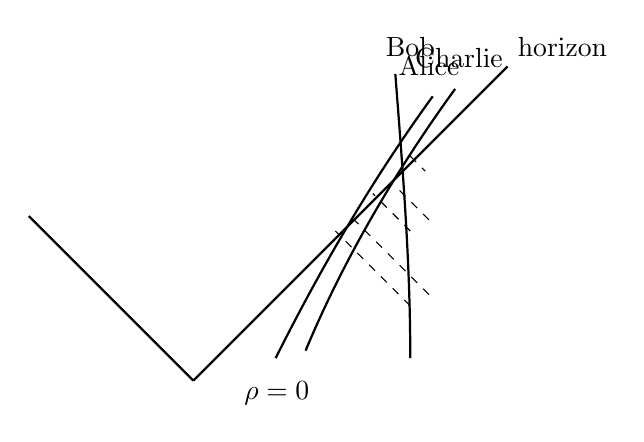
\begin{tikzpicture}[scale=0.95]
\draw[thick] (0,0) -- (4.2,4.2) node[above right] {horizon};
\draw[thick] (0,0) -- (-2.2,2.2);
\draw[thick] (2.9,0.3) .. controls (2.9,1.6) and (2.8,2.8) .. (2.7,4.1);
\draw (2.9,4.2) node[above] {Bob};
\draw[thick] (1.1,0.3) .. controls (1.7,1.5) and (2.4,2.7) .. (3.2,3.8);
\draw (3.15,3.95) node[above] {Alice};
\draw[thick] (1.5,0.4) .. controls (2.0,1.6) and (2.7,2.8) .. (3.5,3.9);
\draw (3.55,4.05) node[above] {Charlie};
\draw[dashed] (2.9,1.0) -- (1.9,2.0);
\draw[dashed] (2.9,2.0) -- (2.4,2.5);
\draw[dashed] (2.9,3.0) -- (3.1,2.8);
\draw[dashed] (3.15,1.15) -- (2.15,2.15);
\draw[dashed] (3.15,2.15) -- (2.75,2.55);
\draw (0.55,0.12) node[below right] {\(\rho=0\)};
\end{tikzpicture}
\caption{Simplified causal construction. The rule is to answer each observer question by drawing the null rays between the worldlines.}
\end{figure}

By the end of the lecture the method has become explicit: do not try to answer these questions by verbal symmetry alone. Draw the diagram. Draw the light rays. Read causality directly from the picture.

\section{What The Diagram Does And Does Not Yet Answer}

The lecture is equally careful about scope. The diagram is powerful, but it is not the whole story of realistic black hole formation.

First, Susskind says that only the upper-right portion of the idealized diagram is physically relevant for a real black hole formed by collapse. The lower half and the apex of the full eternal diagram are not to be taken as literal features of an astrophysical collapse. So one should not overinterpret the complete mathematical extension.

Second, if matter falls in and appreciably changes the mass, then the Schwarzschild radius changes as well. The lecture explicitly postpones the detailed treatment of how the horizon forms and how it grows. We are told only the rough qualitative picture: if one drops in a sufficiently heavy object, the horizon bulges outward, merges, and then relaxes toward a slightly larger sphere. That is a topic for the next lecture, not for the present derivation.

Third, astrophysical light from black holes is not light emitted by the horizon itself. It comes from outside the horizon: accretion disks, hot matter, photons orbiting in complicated ways, and collisions in the surrounding region. So the idealized empty-space Schwarzschild picture should not be confused with the observational appearance of an active black hole.

Fourth, rotation changes the geometry. The lecture touches this only briefly, but enough to mark the boundary: rotating black holes are not described by the simple spherically symmetric picture we have been using, and their horizons and singularities are correspondingly more complicated.

Finally, the lecture returns to the scaling that opened the whole discussion. The causal diagram, once expressed in dimensionless variables, does not change shape when \(r_{\mathrm S}\) changes. What changes is the meaning of distances and times measured on it. The number of meter sticks between two points, or the amount of proper time represented by a segment, scales with \(r_{\mathrm S}\). So a one-kilometer black hole and a \(10^9\)-solar-mass black hole can share the same dimensionless diagram while representing utterly different physical scales.

\section{Summary}

The lecture has a clean spine. We rescale the Schwarzschild metric so that every black hole shares the same dimensionless geometry up to the overall factor \(r_{\mathrm S}^2\). We then use dimensional analysis to see that curvature at the horizon is of order \(1/r_{\mathrm S}^2\), which explains why large black holes have weak horizon tidal forces. Next we replace the coordinate \(r\) by the proper-distance variable \(\rho\), define \(\omega=t/2\), and rewrite the near-horizon metric so that its radial-time part becomes flat spacetime in hyperbolic polar coordinates.

Once that geometry is in hand, the causal story becomes readable. The horizon is not a point but a null line. The interior is the region \(r<1\), and every future-directed timelike or null trajectory inside it hits the true singularity at \(r=0\) in finite proper time. Bob, who remains outside, never sees Alice cross the horizon. Alice feels nothing special at crossing. Charlie, if he free-falls behind her, also sees nothing special there. The rule the lecture leaves us with is the right one: when asked who sees what, draw the diagram and follow the light rays.